\section{系统设计}
\subsection{本章概述}
系统设计将需求分析结果转换为可实现的数据模型和系统结构。本章包括概念结构设计、E-R 图、逻辑结构设计、关系模式、系统功能模块图和其它设计图，保证概念模型、逻辑结构、系统接口和运行界面之间保持一致。

\subsection{概念结构设计说明}
概念结构设计阶段主要根据访客预约、审批流转、门岗通行和统计查询等业务过程抽取实体与联系。核心业务部分包括访客、预约申请、审批记录、通行凭证、出入校记录、黑名单和校门等实体；权限管理部分包括系统用户、角色、权限及其授权关系；系统支撑部分包括通知消息、操作日志、数据字典、截图记录和材料归档记录等实体。各实体围绕“访客提交预约申请”这一主线展开，能够覆盖从预约提交、审批确认、通行核验到访问归档的完整过程。
\begin{longtable}{>{\raggedright\arraybackslash}p{0.300\textwidth}>{\raggedright\arraybackslash}p{0.640\textwidth}}
\caption{主要实体及存在原因}\\
\toprule
实体 & 存在原因 \\
\midrule
visitor & 保存访客身份基础信息，避免同一访客多次预约时重复录入。 \\
visit\_apply & 保存预约申请主记录，连接访客、被访人、部门、车辆、审批和出入校流程。 \\
approval\_record & 保存被访人确认、部门审批等多阶段审批过程。 \\
pass\_code & 保存审批通过后的通行凭证和有效期。 \\
access\_record & 保存门岗核验后的入校、离校和异常记录。 \\
blacklist & 保存限制或风险访客，支撑预约和核验阶段的安全检查。 \\
系统用户 & sys\_user 保存登录账号、真实姓名、联系方式和所属部门。 \\
角色 & sys\_role 保存系统角色及角色状态。 \\
权限 & sys\_permission 保存菜单权限、接口权限和父子权限结构。 \\
operation\_log & 保存关键业务操作日志，支撑审计和测试说明。 \\
\bottomrule
\end{longtable}
\subsection{E-R 图}
为了避免一张图实体过多、线条交叉严重，报告将 E-R 图拆分为总体简化 E-R 图、核心业务 E-R 图、用户权限 E-R 图和系统支撑 E-R 图。正文重点展示总体关系和核心业务关系，权限与支撑实体作为补充说明。
\subsubsection{总体简化 E-R 图}

总体简化 E-R 图只展示主要实体和主流程关系，用于报告正文快速说明系统数据模型全貌。

\begin{figure}[H]

  \centering

  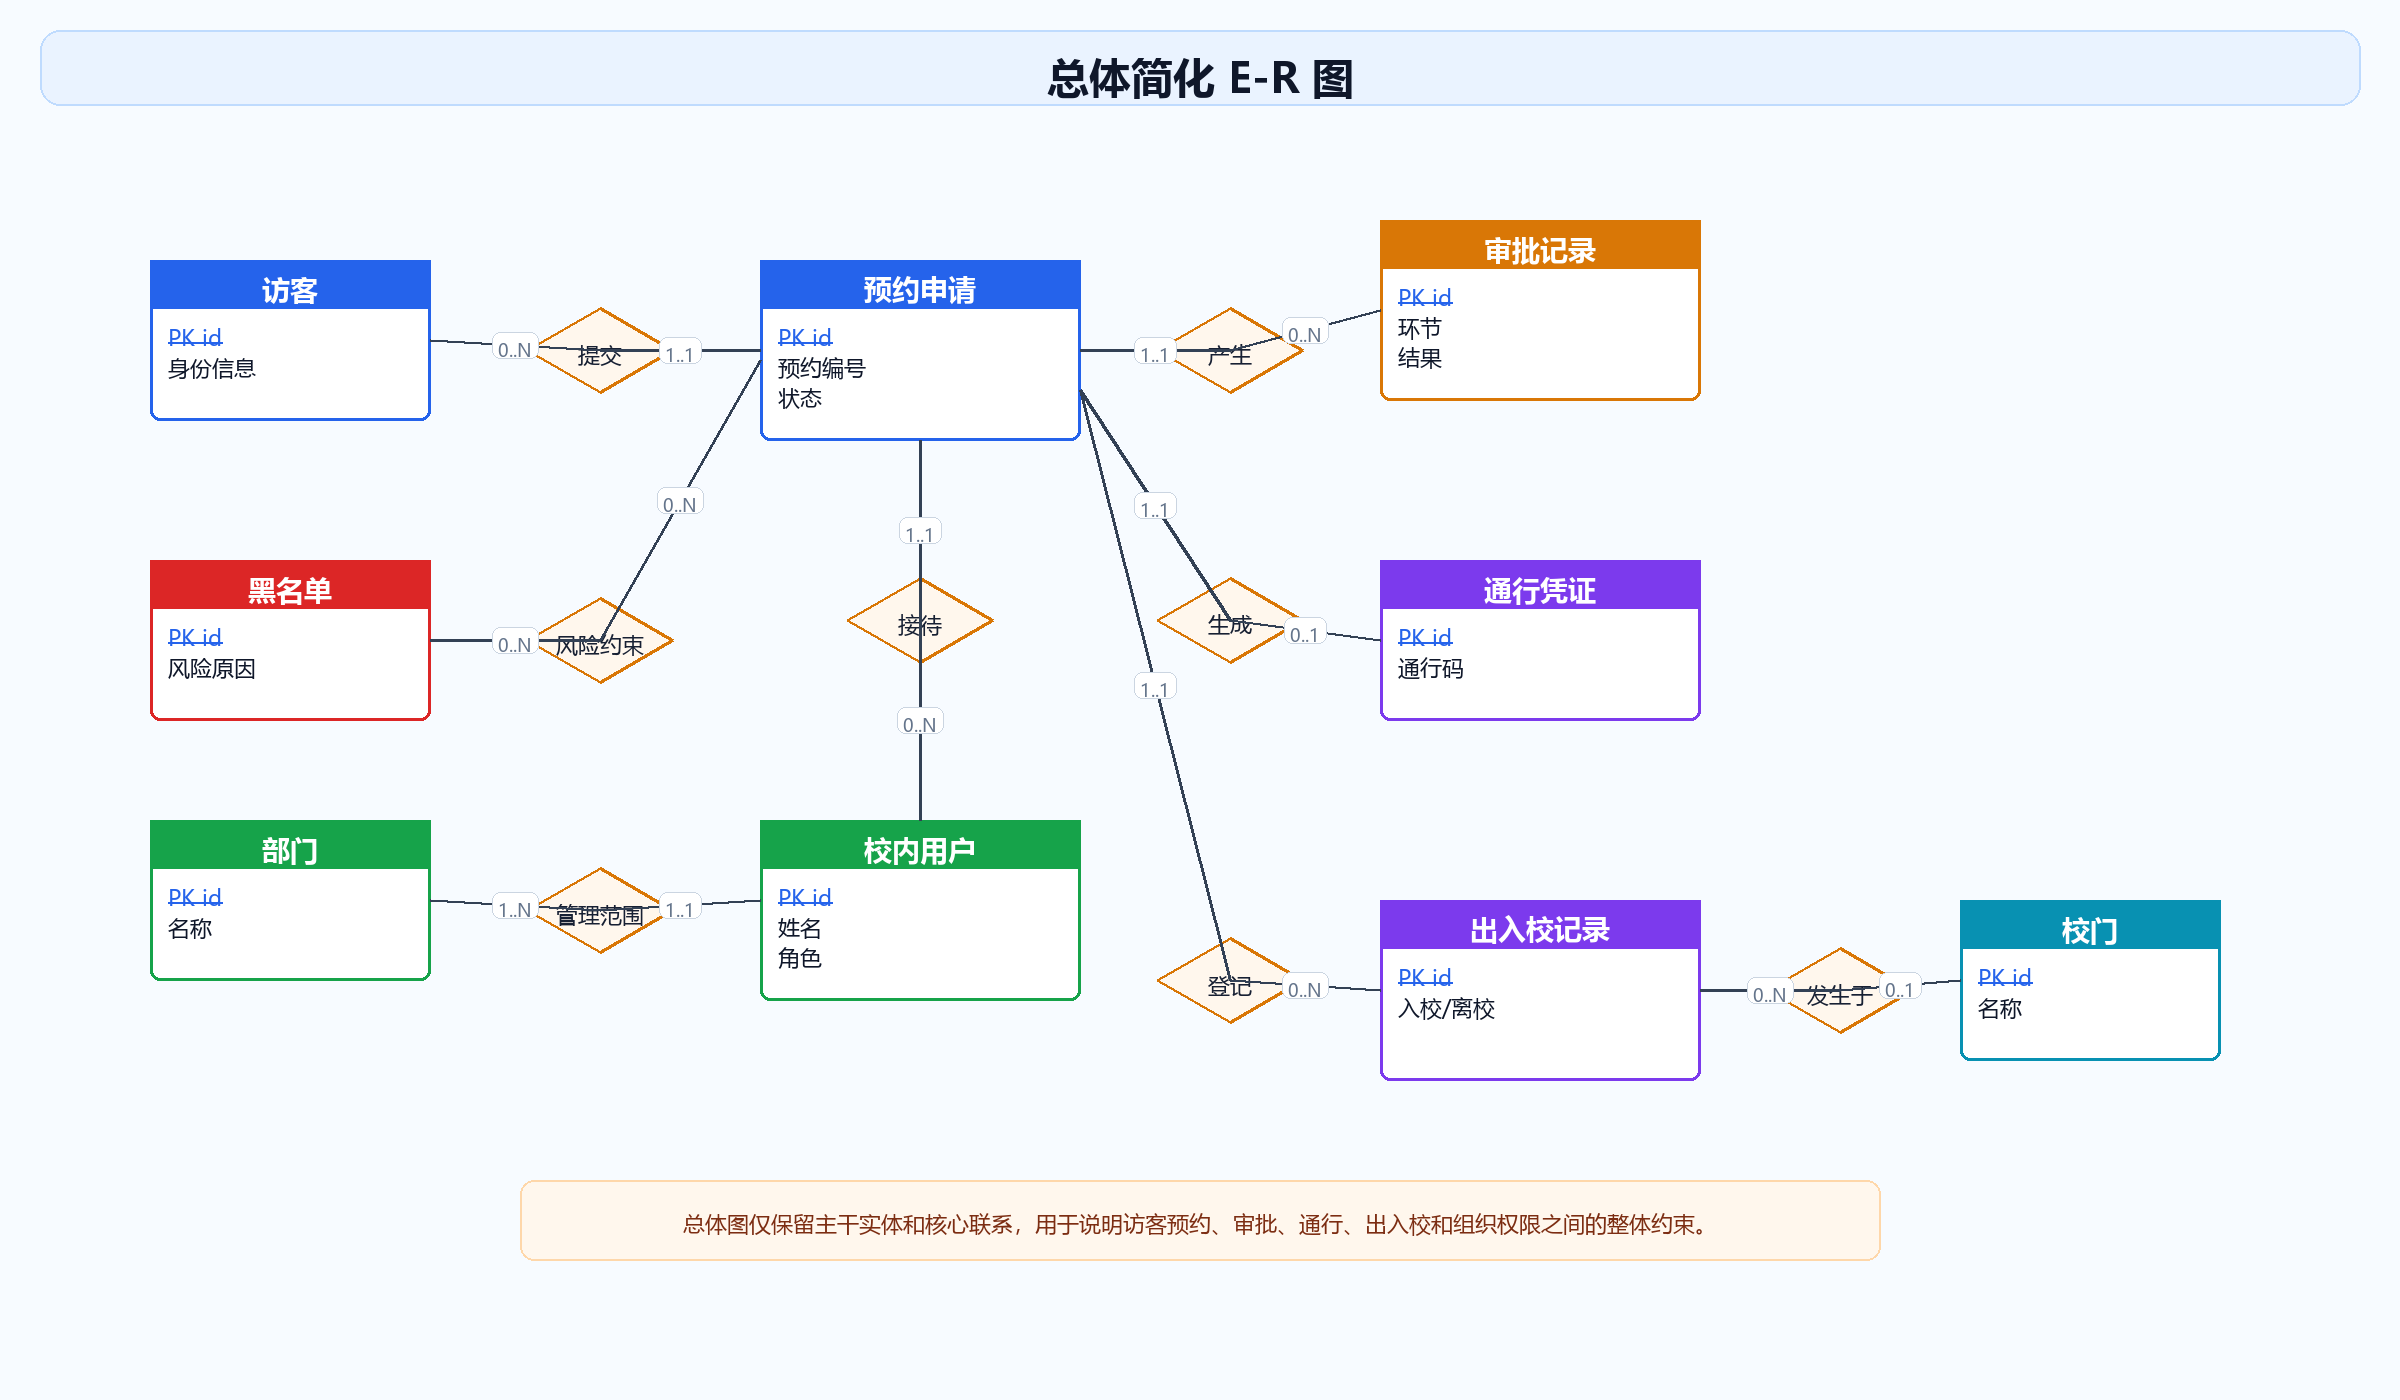
\includegraphics[width=0.94\textwidth]{figures/er_overview.png}

  \caption{总体简化 E-R 图}

\end{figure}\subsubsection{核心业务 E-R 图}

核心业务 E-R 图围绕访客预约、审批、通行凭证、出入校记录和黑名单展开，是后续关系模式转换的主要依据。

\begin{figure}[H]

  \centering

  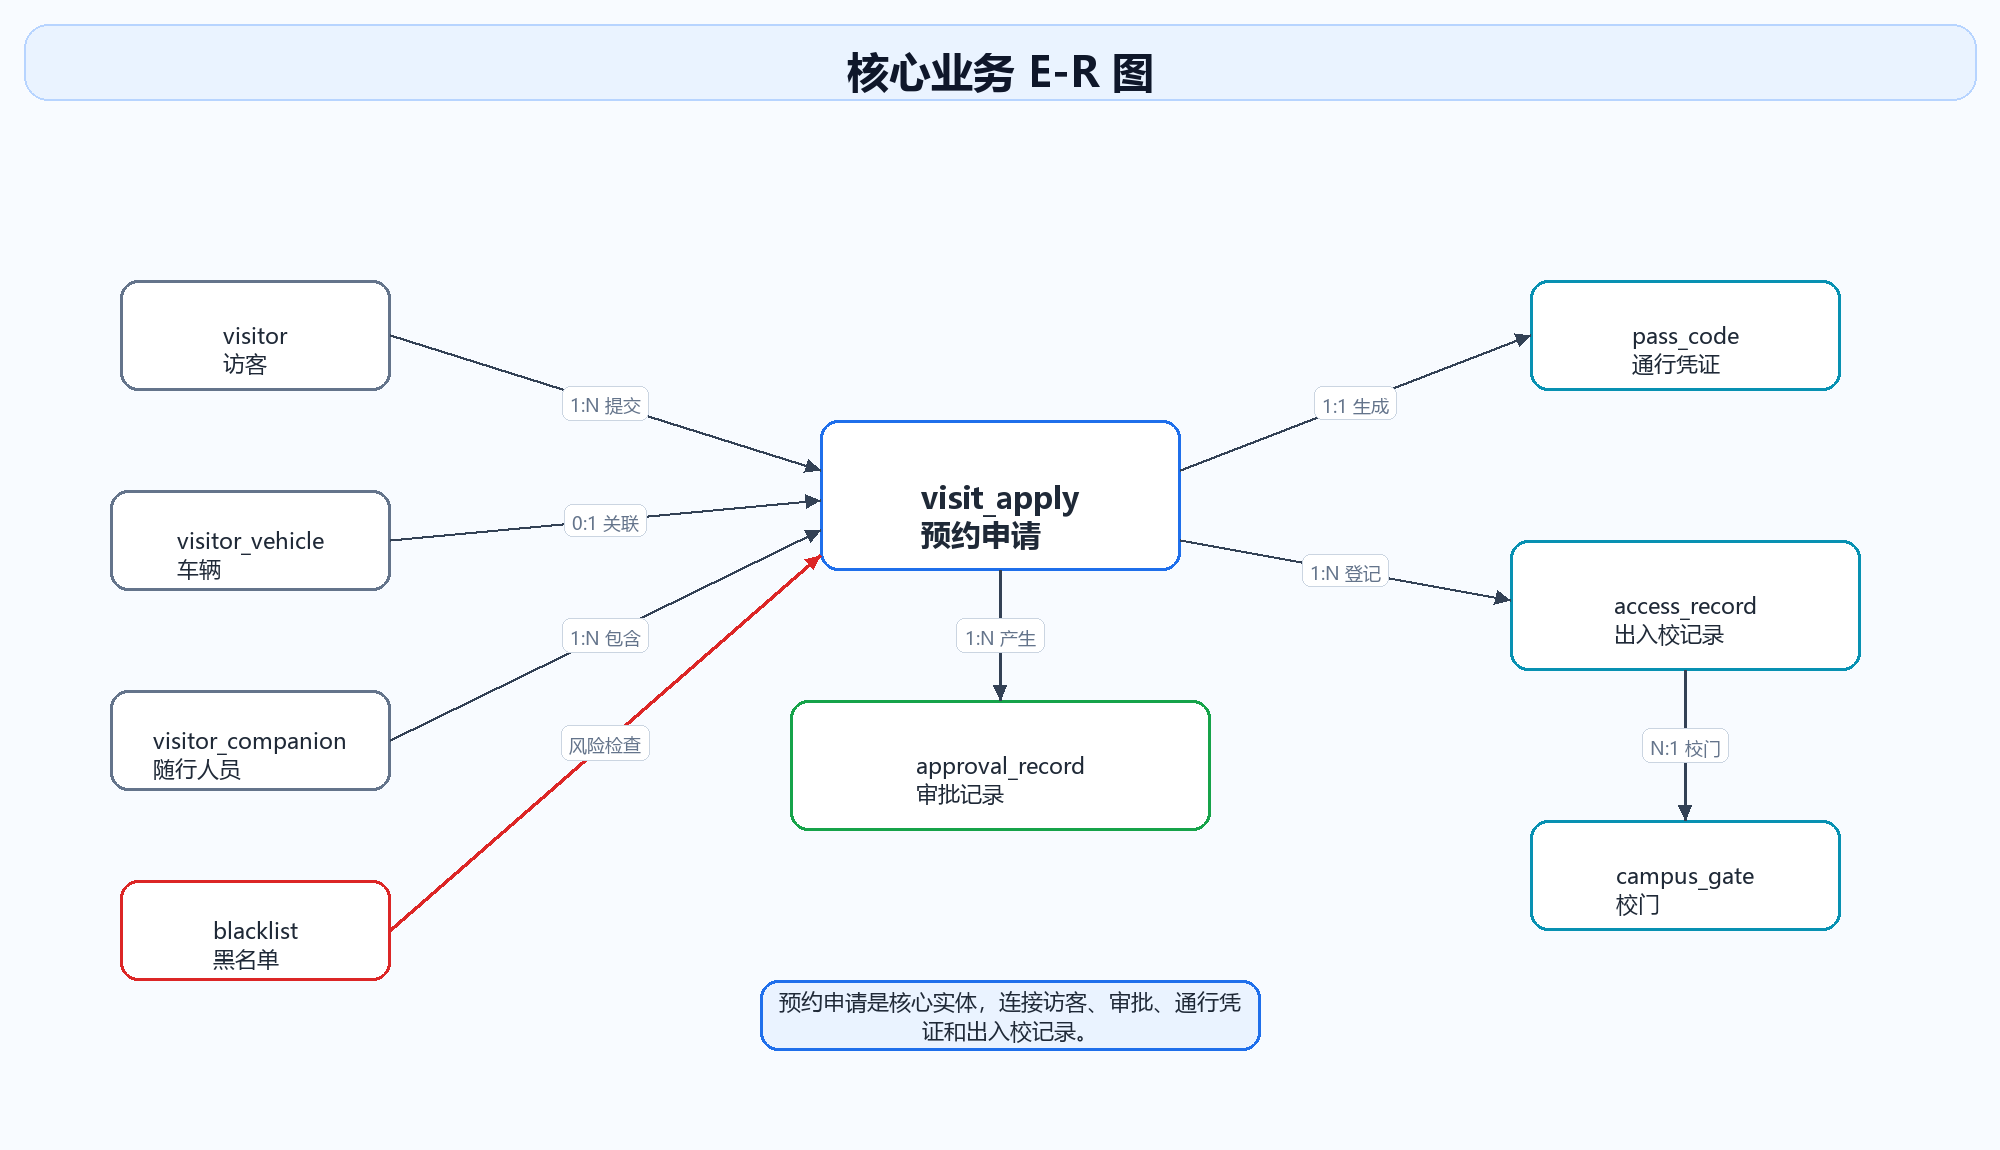
\includegraphics[width=0.94\textwidth]{figures/er_core_business.png}

  \caption{核心业务 E-R 图}

\end{figure}\subsubsection{用户权限 E-R 图}

用户权限 E-R 图展示系统用户、角色、权限、部门及两个多对多中间表之间的联系。

\begin{figure}[H]

  \centering

  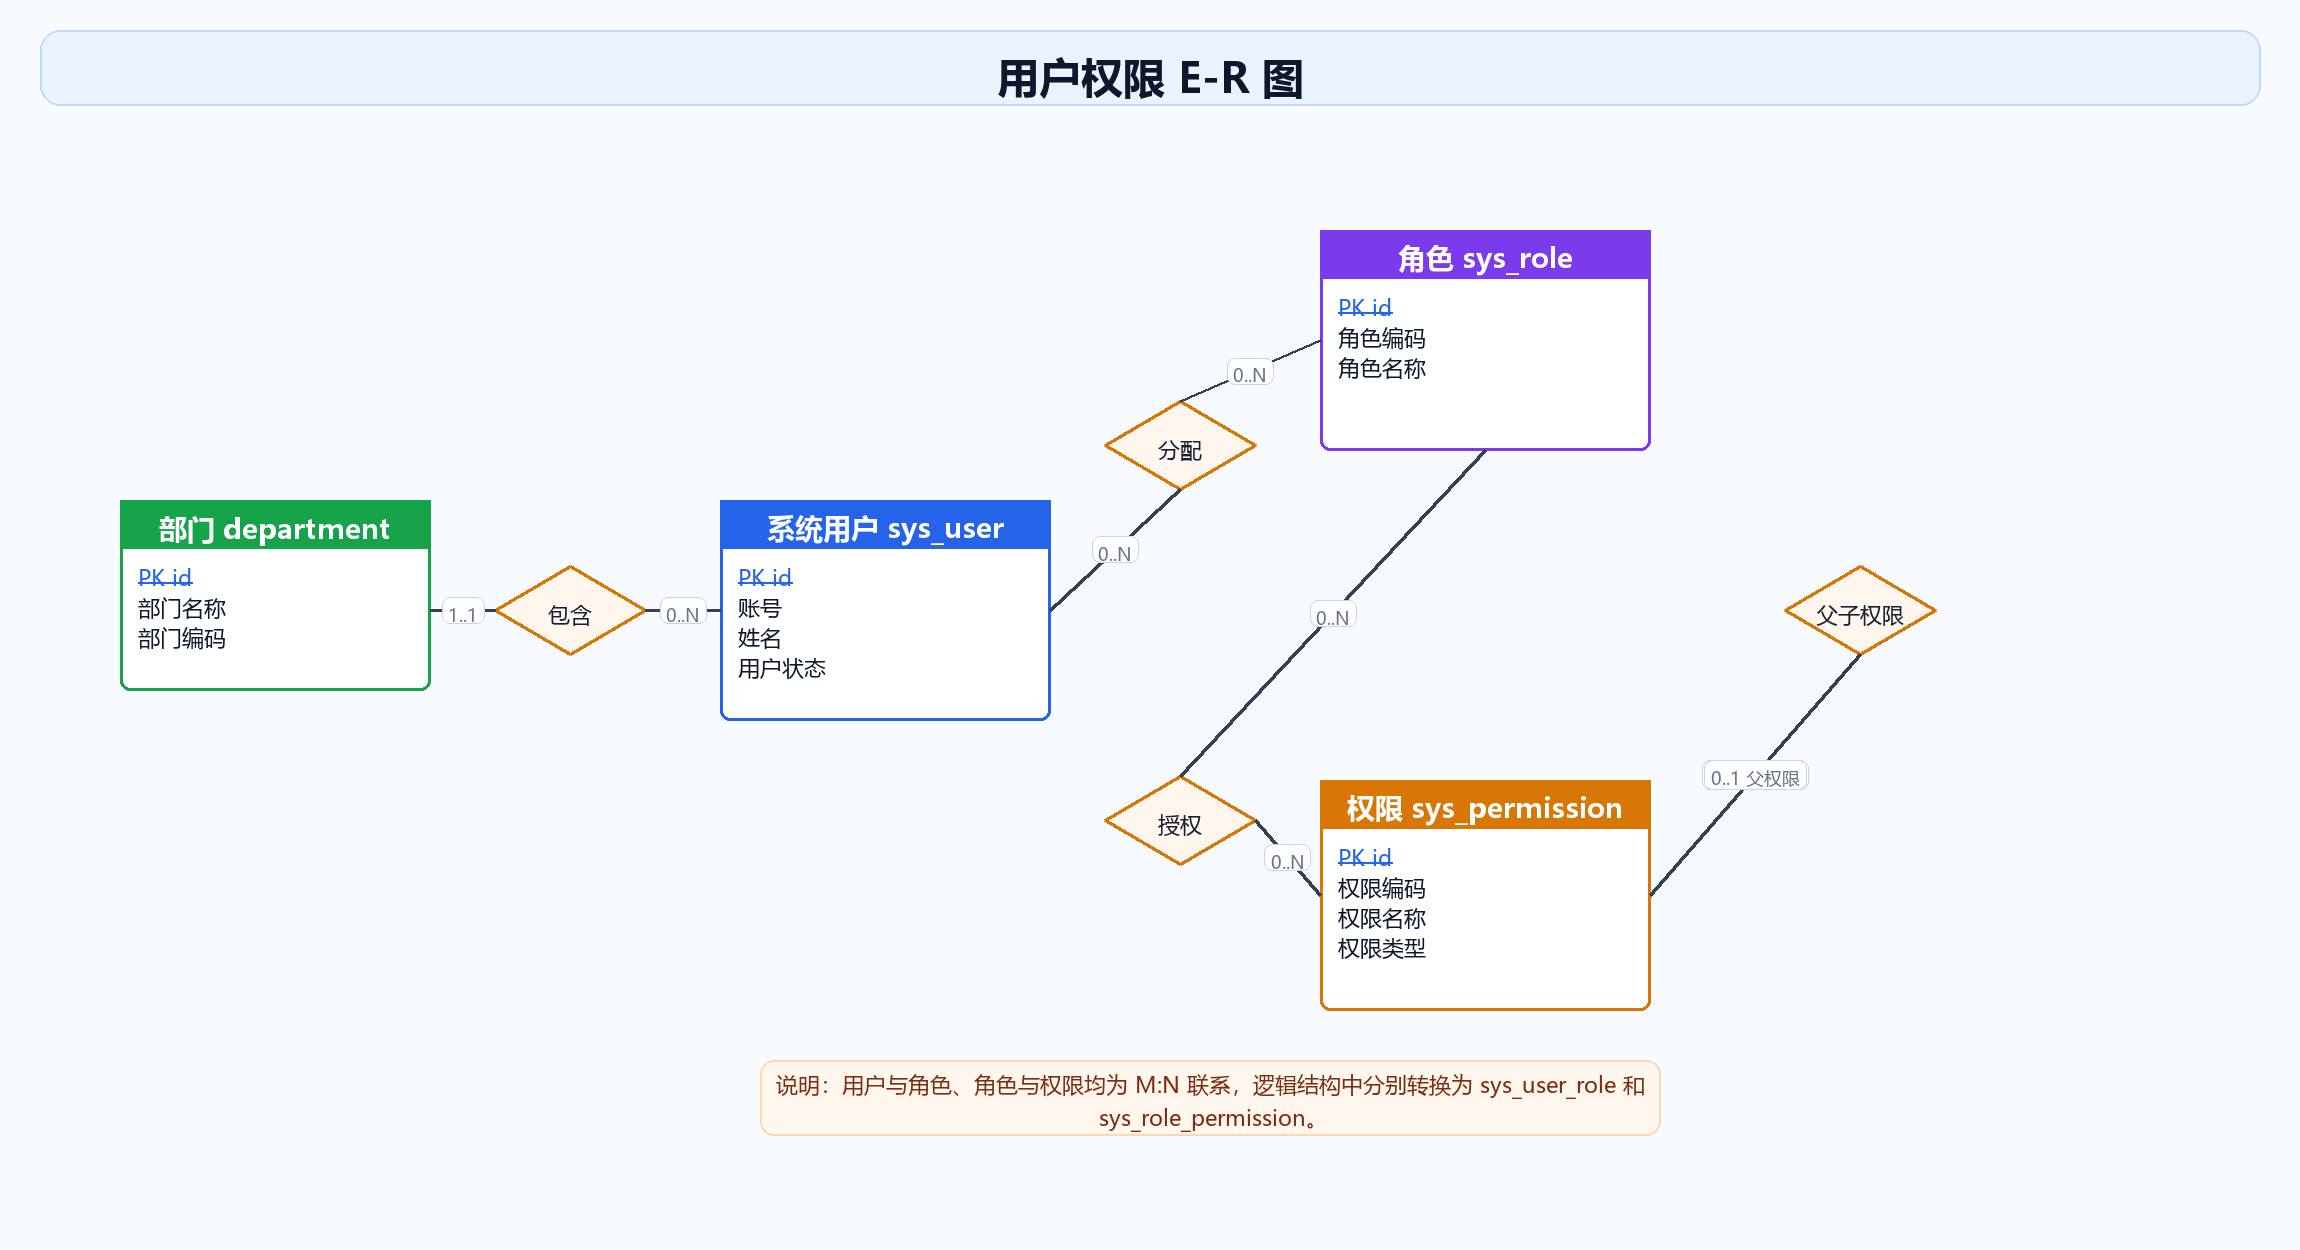
\includegraphics[width=0.94\textwidth]{figures/er_user_permission.png}

  \caption{用户权限 E-R 图}

\end{figure}\subsubsection{系统支撑 E-R 图}

系统支撑 E-R 图展示通知、日志、字典、截图记录和报告记录等支撑性实体。

\begin{figure}[H]

  \centering

  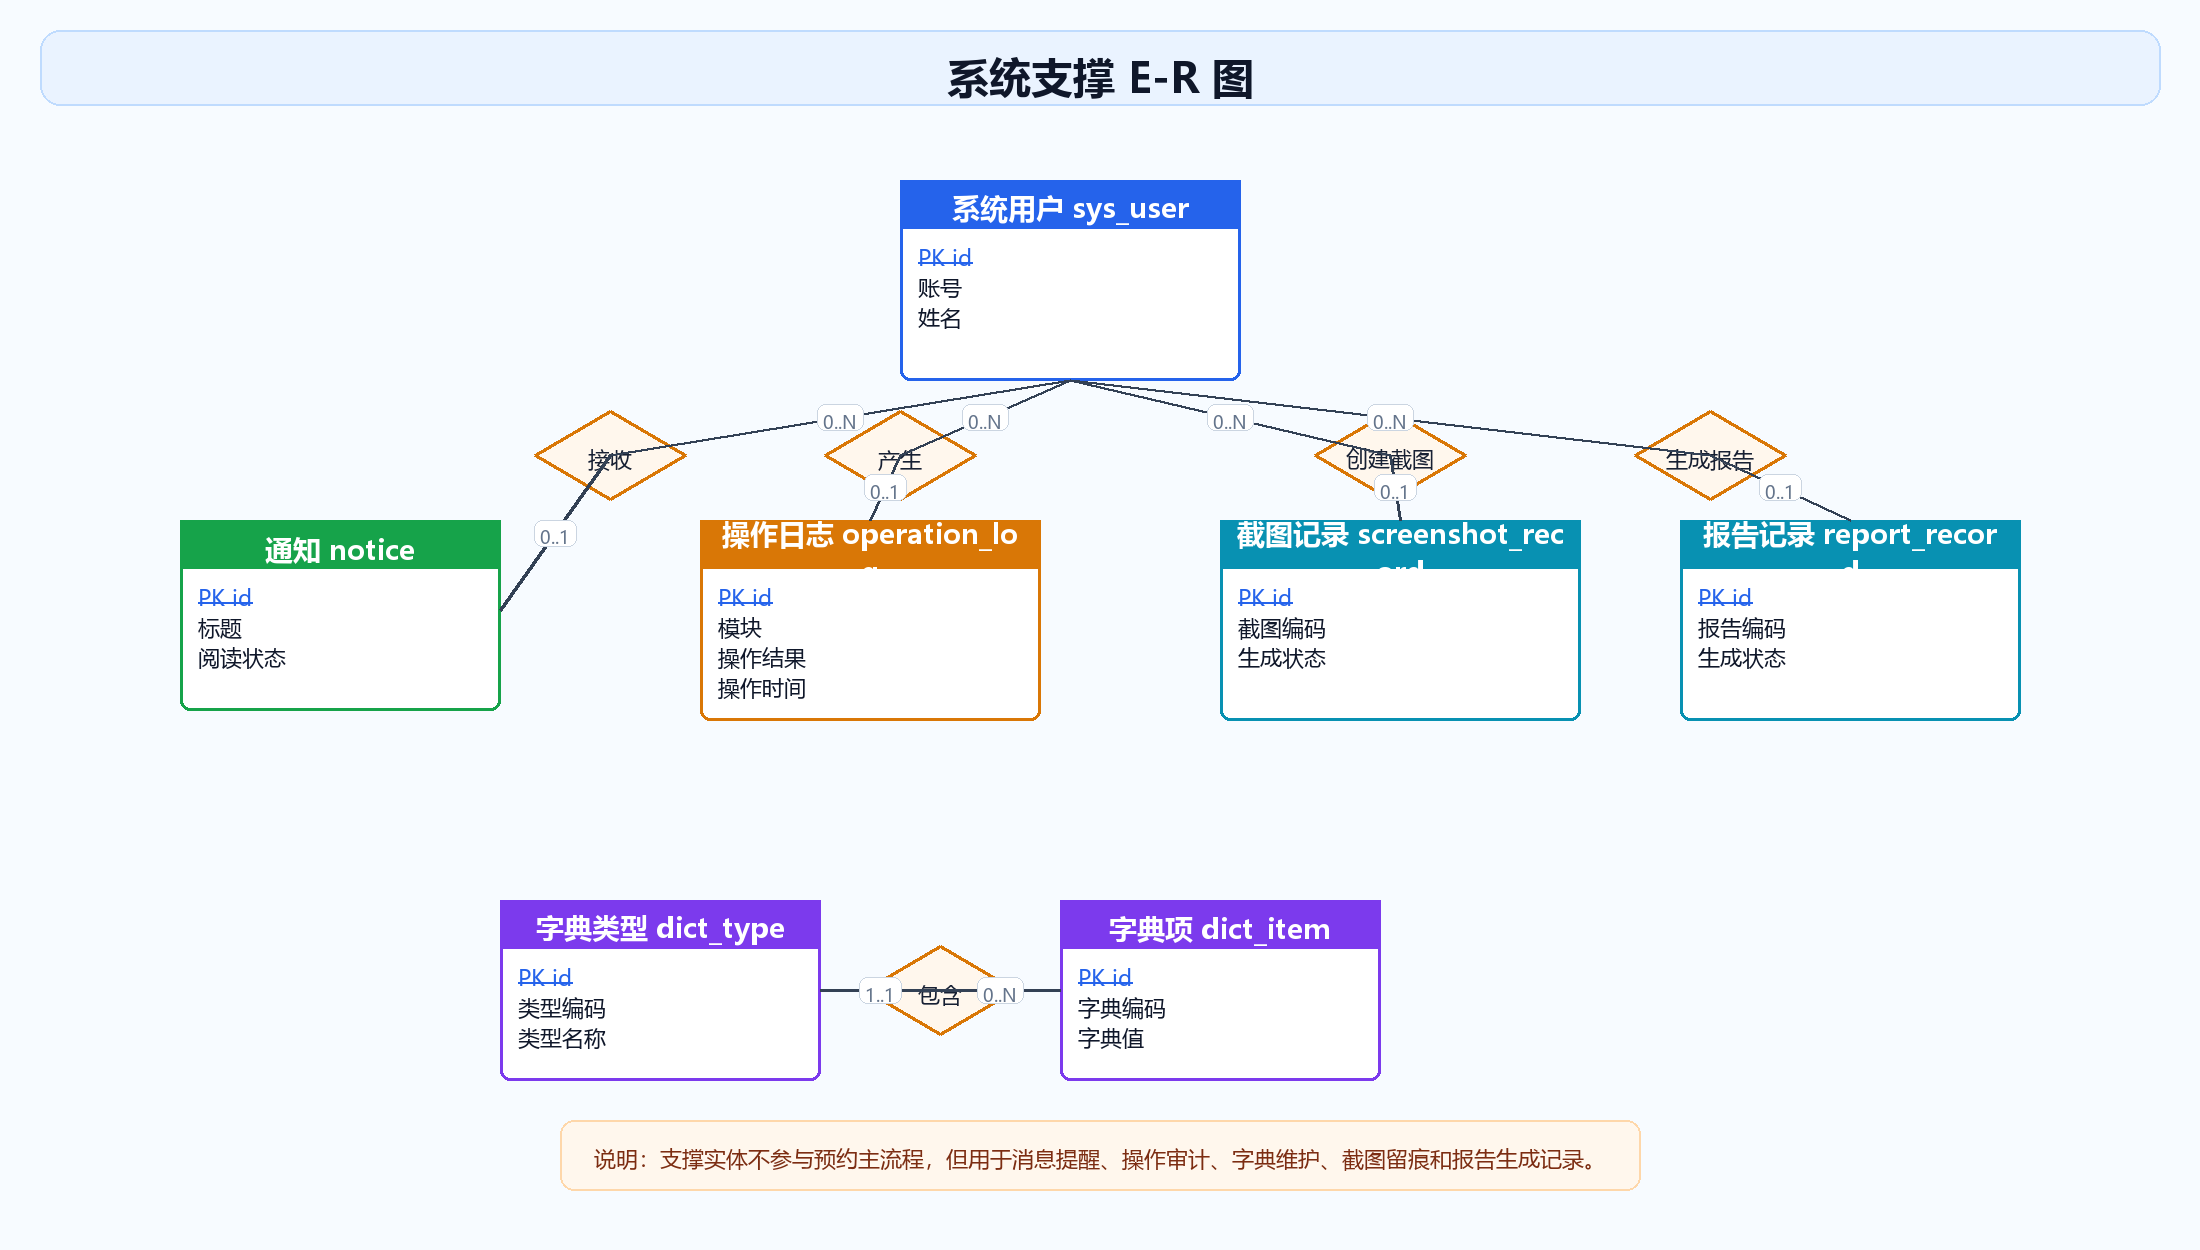
\includegraphics[width=0.94\textwidth]{figures/er_system_support.png}

  \caption{系统支撑 E-R 图}

\end{figure}
\subsection{逻辑结构设计说明}
逻辑结构设计将概念实体转换为 MySQL 关系表。实体表统一使用 \texttt{id} 作为主键，时间字段统一使用 \texttt{create\_time}、\texttt{update\_time}，软删除字段统一使用 \texttt{deleted}。多对多关系通过 sys\_user\_role 和 sys\_role\_permission 中间表表达；一对多关系通过外键字段或业务关联字段表达；预约、审批、通行和出入校状态通过状态字段表达。
\begin{longtable}{>{\raggedright\arraybackslash}p{0.140\textwidth}>{\raggedright\arraybackslash}p{0.270\textwidth}>{\raggedright\arraybackslash}p{0.360\textwidth}>{\raggedright\arraybackslash}p{0.170\textwidth}}
\caption{主要关系表设计摘要}\\
\toprule
设计分组 & 主要关系表 & 设计重点 & 主要约束 \\
\midrule
权限与组织 & 系统用户表、角色表、权限表、用户角色关联表、角色权限关联表、部门表 & 管理登录用户、部门归属、角色授权和菜单接口权限，是系统访问控制的基础。 & 用户与角色、角色与权限均采用中间表表示多对多关系。 \\
访客基础 & 访客表、访客车辆表、随行人员表、黑名单表 & 保存访客身份、车辆、同行人员和风险名单，为预约申请和门岗核验提供基础数据。 & 访客身份、手机号、车辆和黑名单信息参与预约与核验约束。 \\
预约审批 & 预约申请表、审批记录表、通行凭证表 & 保存从提交申请、被访人确认、部门审批到生成通行凭证的核心业务链路。 & 预约编号唯一，审批记录按环节和时间形成完整处理轨迹。 \\
出入校管理 & 出入校记录表、校门表 & 记录门岗核验、入校登记、离校登记、当前在校和超时未离校等访问状态。 & 出入校记录关联预约、访客、通行凭证、校门和安保人员。 \\
消息与日志 & 通知消息表、操作日志表 & 保存预约提醒、审批提醒、风险提醒和关键操作审计记录。 & 通知关联接收人和业务对象，日志记录操作人、模块和处理结果。 \\
字典与材料 & 字典类型表、字典项表、截图记录表、报告记录表 & 维护状态、类型等基础字典，并保存课程展示材料的整理记录。 & 字典项归属于字典类型，材料记录保存编号、路径、状态和时间。 \\
\bottomrule
\end{longtable}
\subsection{关系模式说明}
系统关系模式由概念结构转换得到，重点保持实体、联系和业务约束之间的一致性。访客表保存校外人员身份基础信息；预约申请表保存一次访问申请，并关联访客、被访人、部门、车辆和访问时间；审批记录表保存被访人确认、部门审批等环节的处理结果；通行凭证表保存审批通过后的校验凭证和有效期；出入校记录表保存门岗核验后的入校、离校和异常状态；黑名单表用于记录限制入校或需要重点关注的风险人员。用户、角色和权限之间的多对多关系通过中间表表达，既保证权限控制清晰，也避免在单个实体中重复保存授权信息。

\subsection{系统功能模块图}
系统功能模块图按角色和业务域划分为访客端、被访人端、审批管理、门岗管理、访客记录、安全管理、统计报表、系统管理和系统支撑等模块。
\subsubsection{系统功能模块图}

模块图展示系统功能分解及各模块边界，便于说明前端菜单、后端接口和权限控制的对应关系。

\begin{figure}[H]

  \centering

  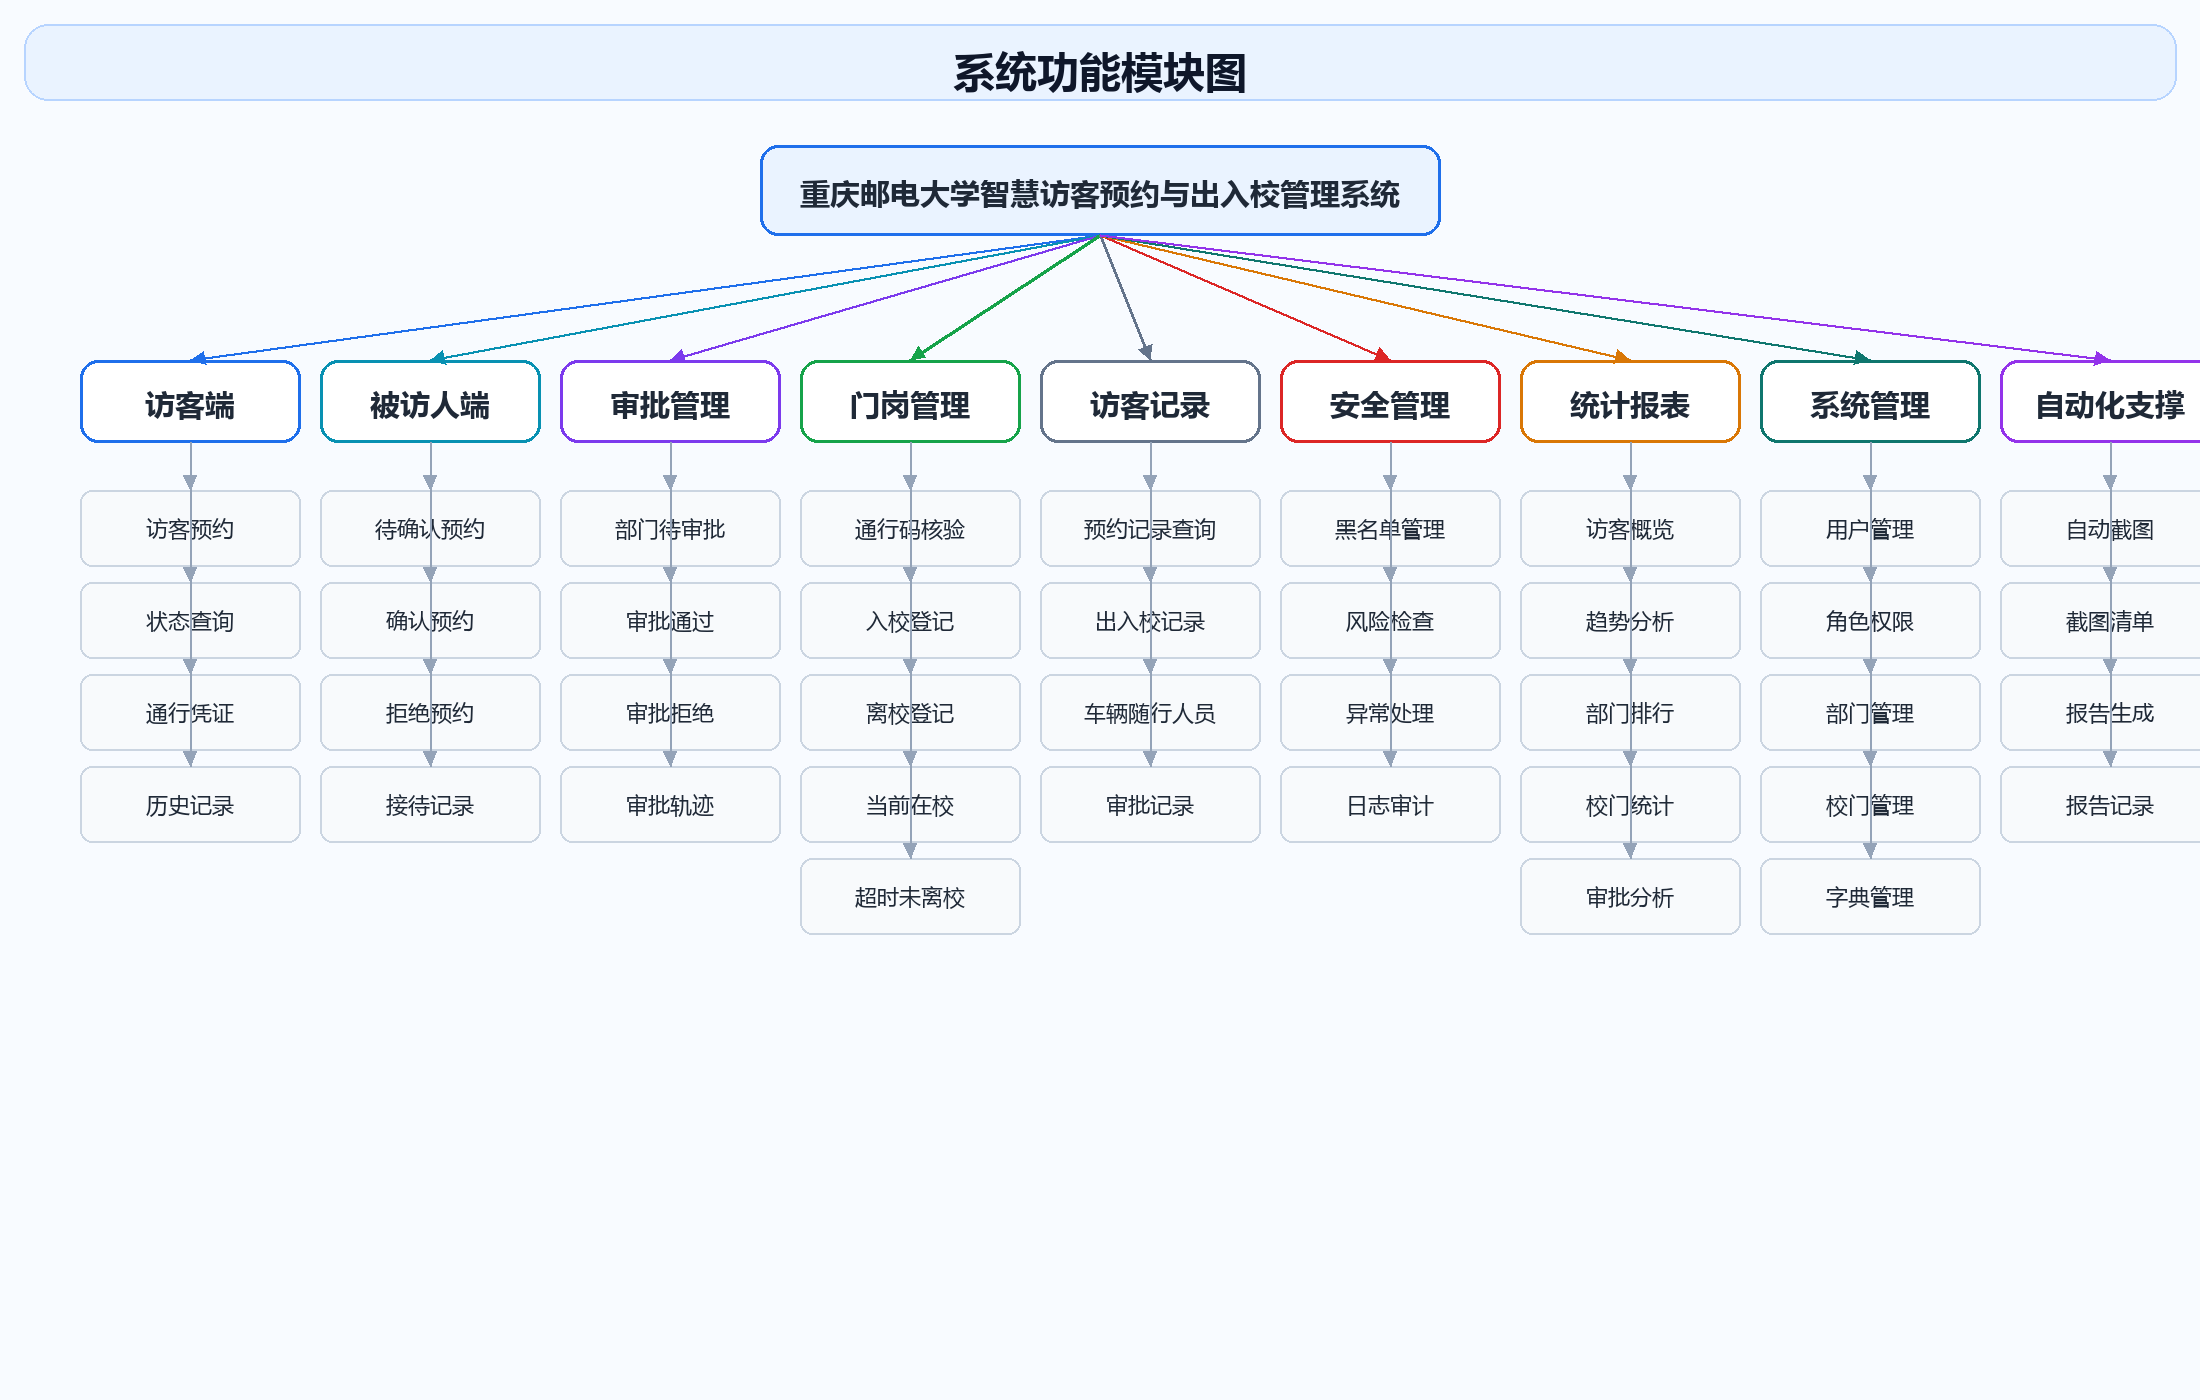
\includegraphics[width=0.94\textwidth]{figures/system_module.png}

  \caption{系统功能模块图}

\end{figure}\subsection{其它设计图}\subsubsection{访客预约审批流程图}

访客预约审批流程图展示从预约提交到审批通过或拒绝的状态流转，并体现黑名单拦截、被访人拒绝和部门审批拒绝等异常分支。

\begin{figure}[H]

  \centering

  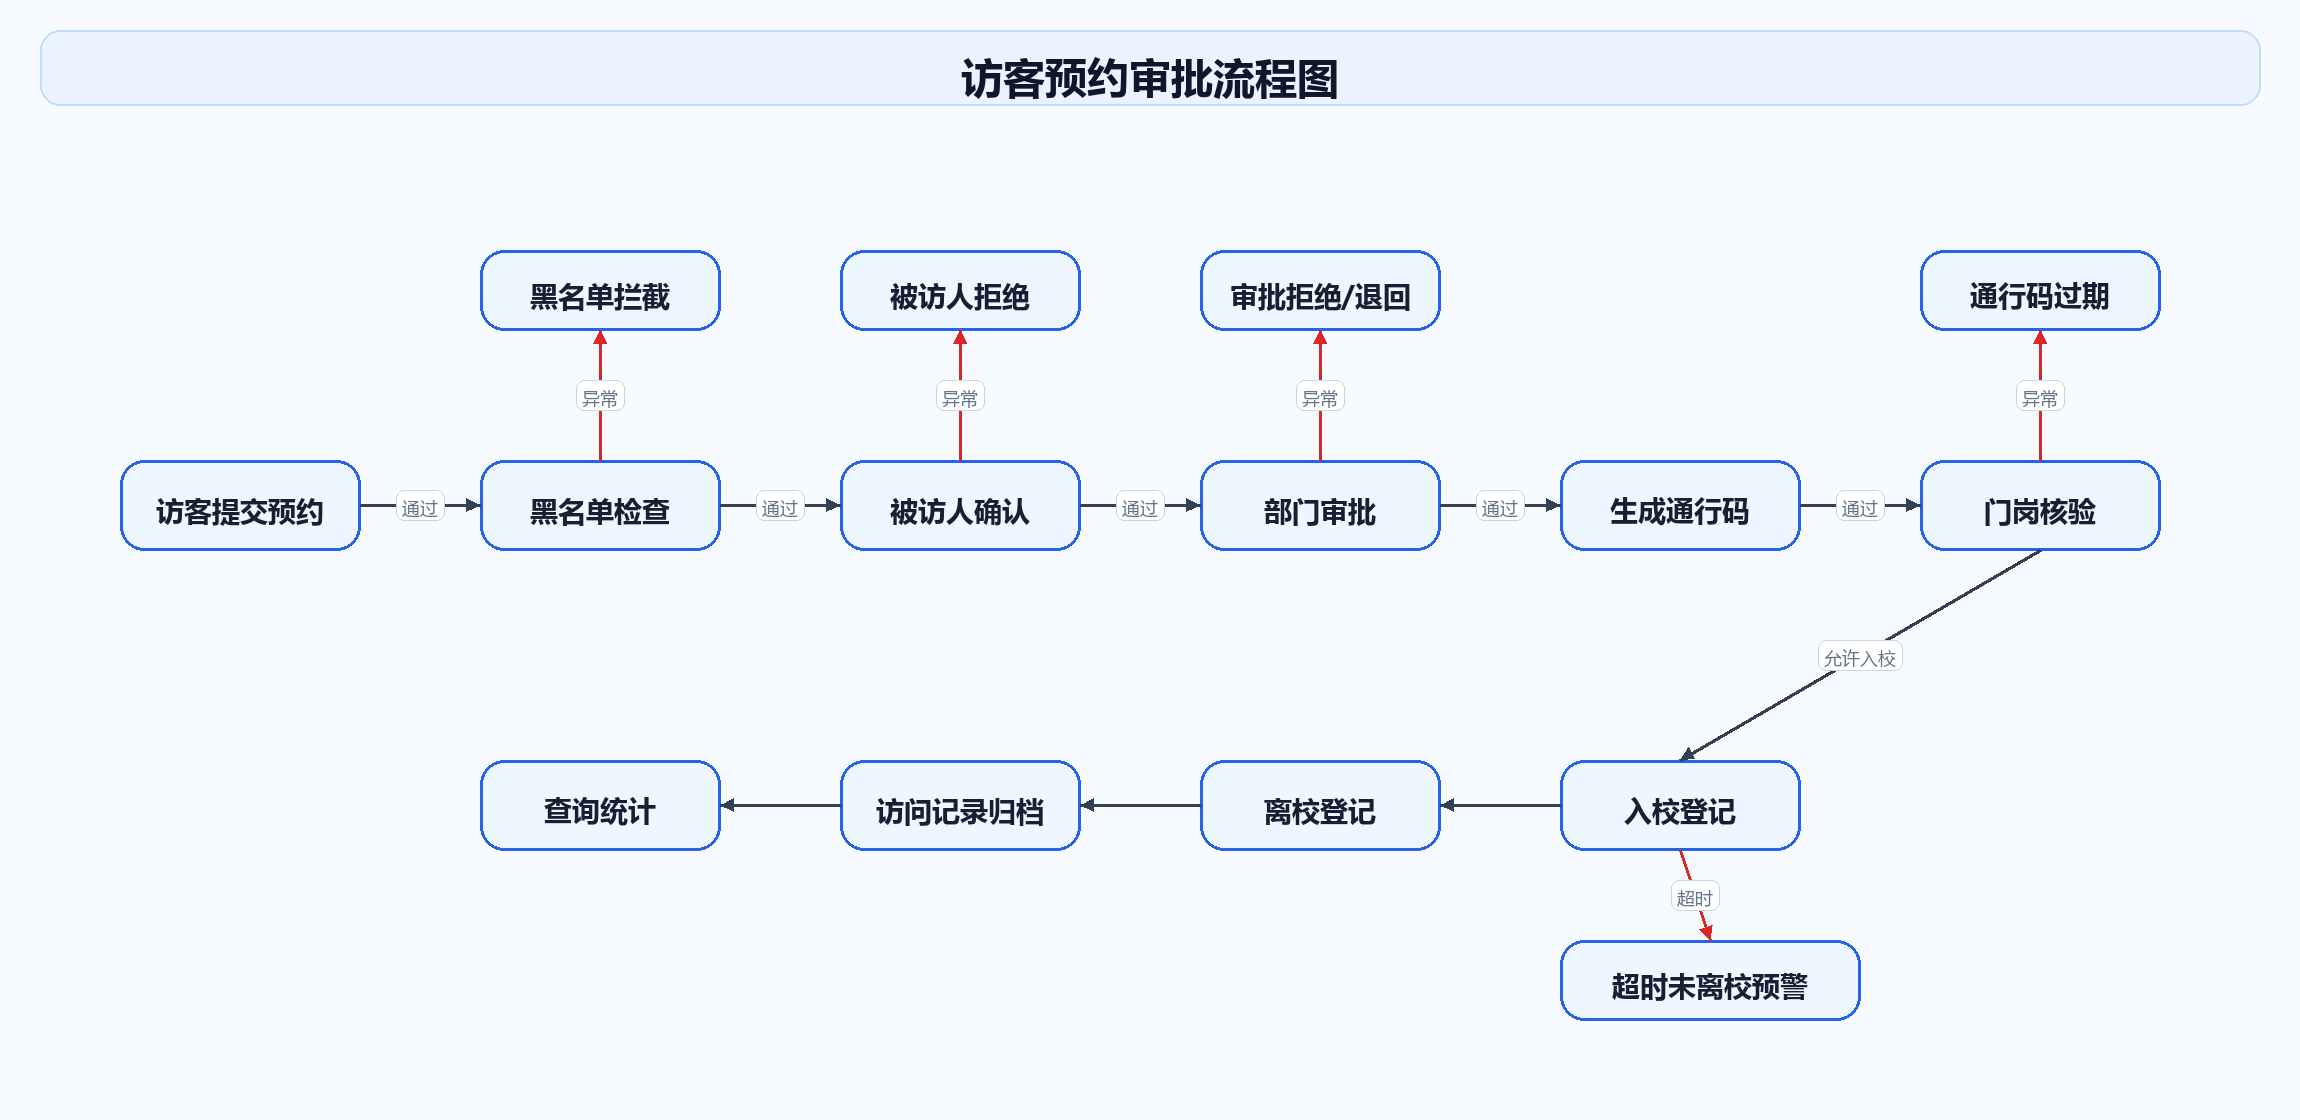
\includegraphics[width=0.94\textwidth]{figures/visitor_workflow.png}

  \caption{访客预约审批流程图}

\end{figure}\subsubsection{门岗核验入校流程图}

门岗核验流程图展示通行码核验、时间有效性检查、黑名单检查、入校登记、离校登记和超时未离校处理。

\begin{figure}[H]

  \centering

  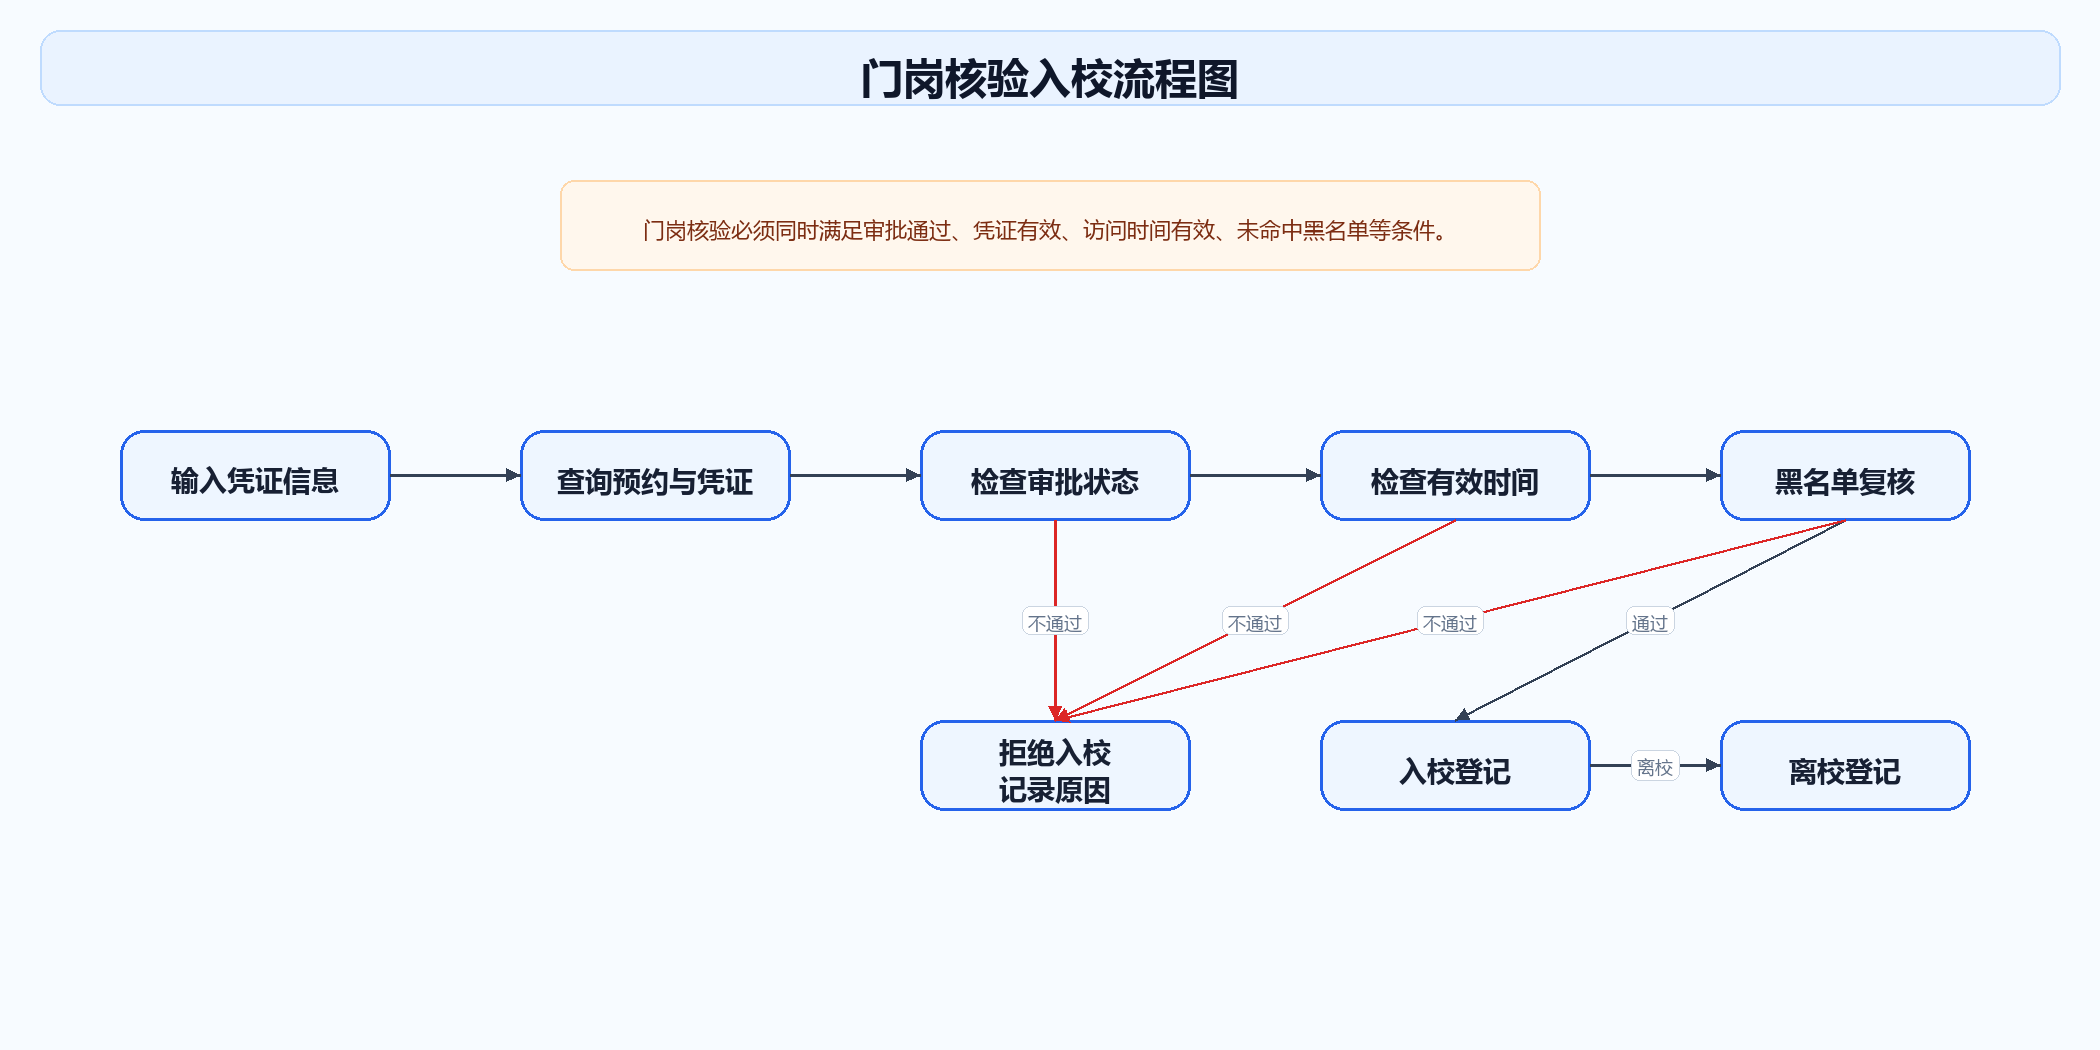
\includegraphics[width=0.94\textwidth]{figures/gate_check_workflow.png}

  \caption{门岗核验入校流程图}

\end{figure}\subsubsection{系统架构图}

系统架构图展示浏览器前端、Spring Boot 后端、MySQL 数据库、运行界面截图和课程设计材料之间的关系。

\begin{figure}[H]

  \centering

  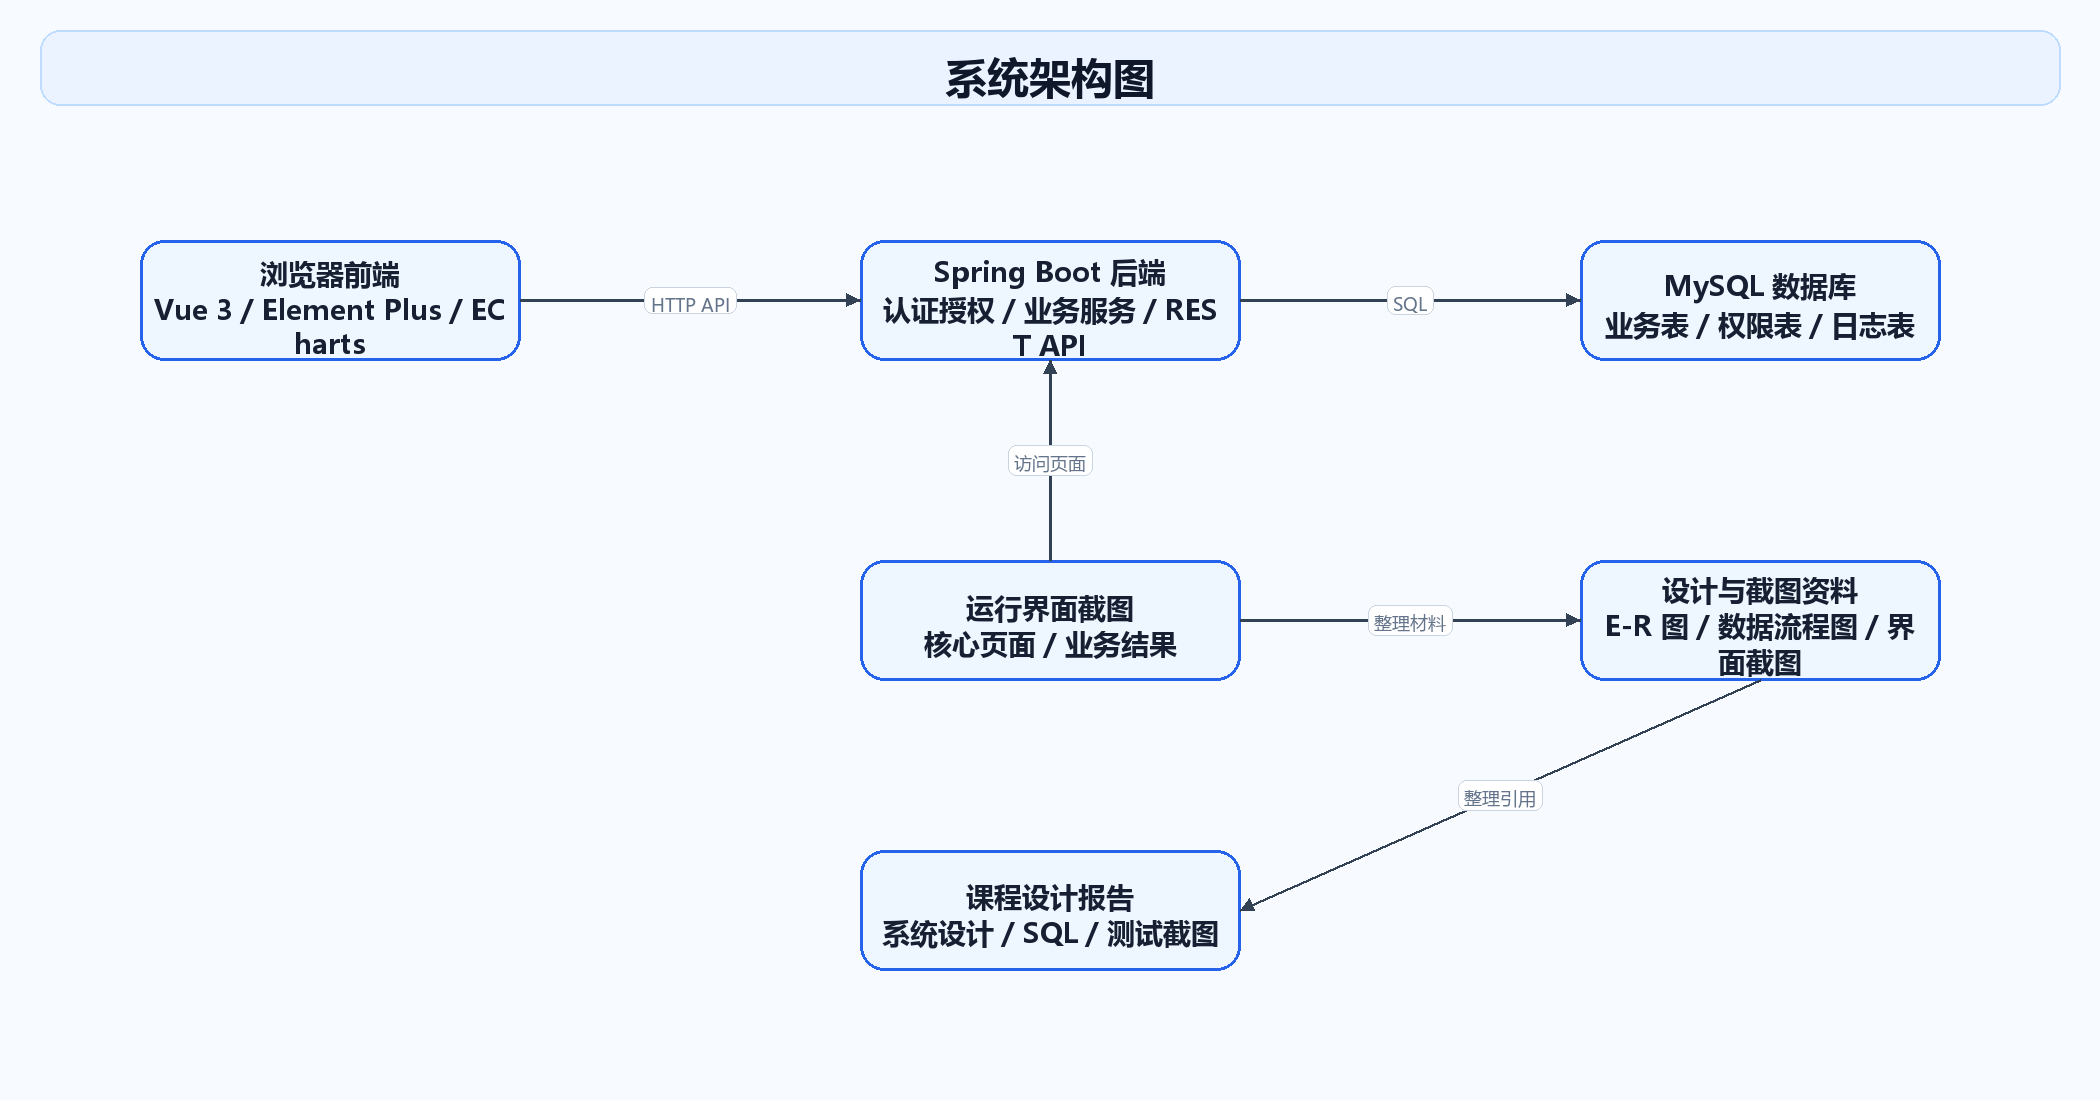
\includegraphics[width=0.94\textwidth]{figures/system_architecture.png}

  \caption{系统架构图}

\end{figure}\subsubsection{数据库表关系图}

数据库表关系图适合放入附录，用于展示主外键关系和表间依赖。

\begin{figure}[H]

  \centering

  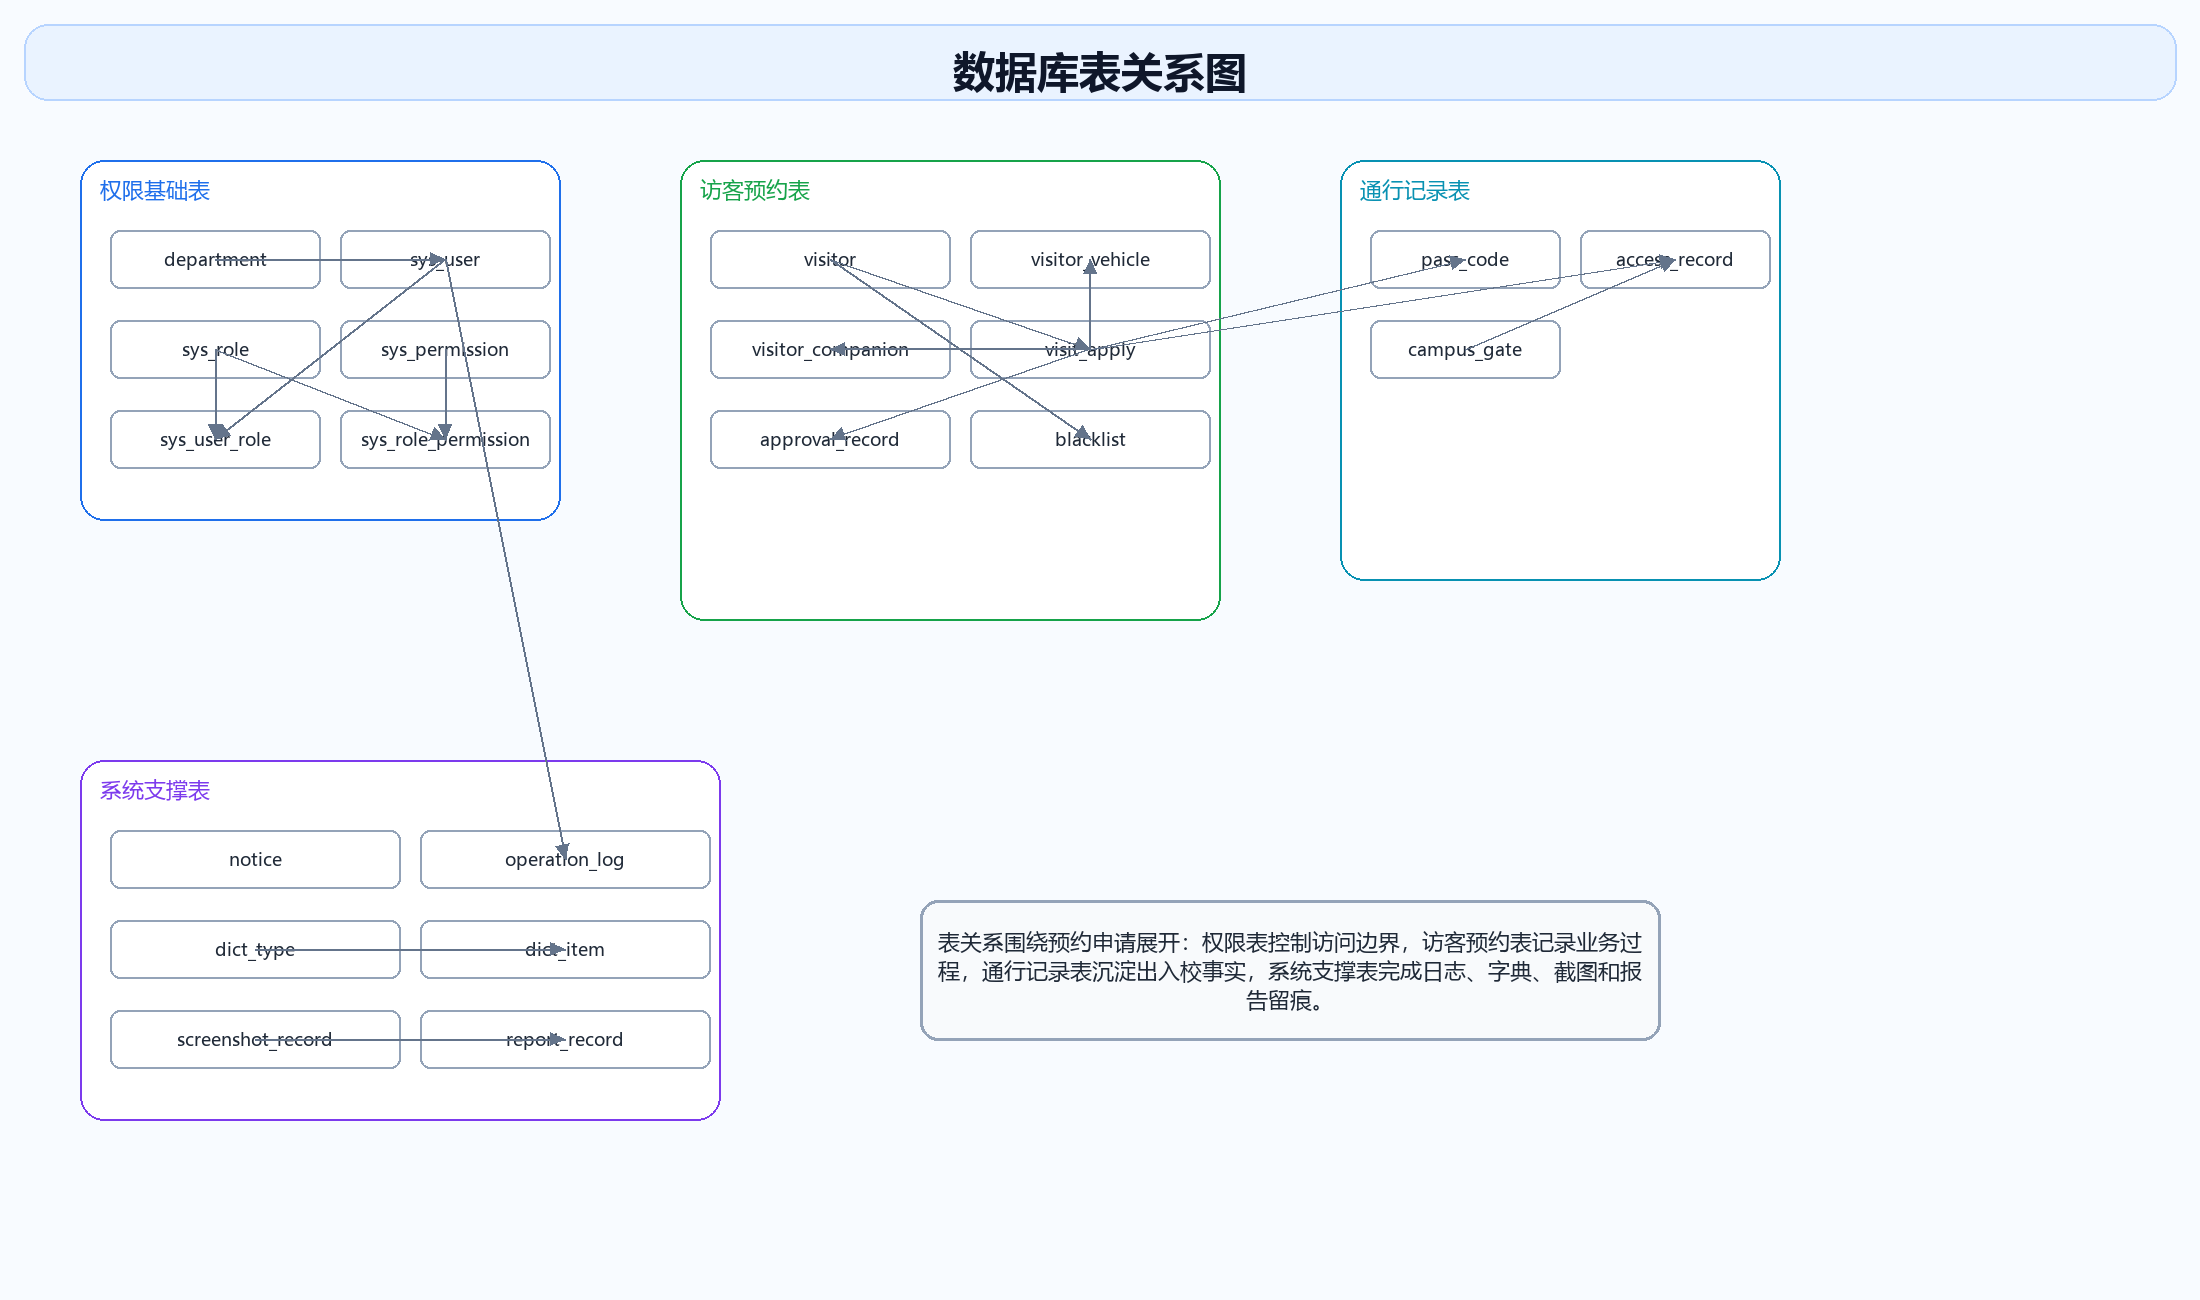
\includegraphics[width=0.94\textwidth]{figures/table_relation.png}

  \caption{数据库表关系图}

\end{figure}
